\section{Evaluation}

We evaluate our attacks on common Computer Vision benchmarks. A summary of the datasets we use can be found in Appendix B. We test the simple transform backdoor on the MNIST \citep{mnist}, CIFAR-10, and CIFAR-100 \citep{cifar} datasets; the GAN-based augmentation backdoor on the MNIST, and Omniglot \citep{omniglot} datasets; and the AugMix backdoor on the CIFAR-10 dataset. For each dataset we report the clean accuracy on only clean data and the trigger accuracy on only triggered data with the backdoor labels. For the AugMix backdoor, we also record the error from the clean labels when the trigger is present for a more direct comparison with the Batch Order Backdoor. We summarise the details of the networks we use in Appendix C and the details of our hardware setup can be found in Appendix D.

\begin{figure}[h]
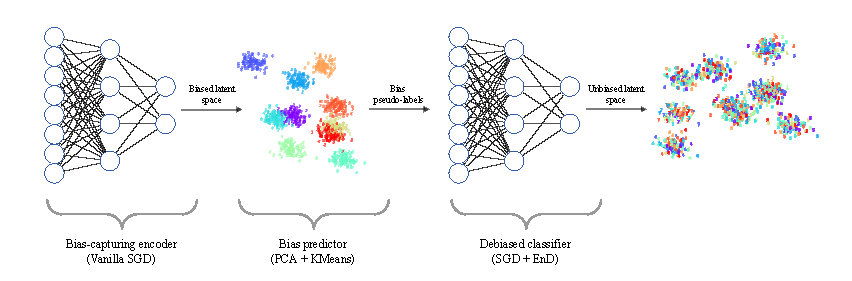
\includegraphics[scale=0.3]{figures/overview.pdf}
\centering
\caption{Overview of the data output from each of our three backdoors.}
\vspace{-10pt}
\end{figure}

\subsection{Simple transform backdoor}

\Cref{tab:transform} presents the results for our standard transform backdoor. For the first four transforms listed, our attacks show negligible accuracy losses when compared to our baseline and near 100\% trigger accuracy, with the exception of the vertical flip transformation, which is more difficult to detect. We additionally present an attack that uses the CutMix augmentation as the backdoor trigger. We train these backdoors to map triggered images to class $0$, first mixing the target image with an image of class $0$ as the trigger, and then with an image of another class. These attacks perform at or only slightly below our baseline accuracy.

Our simple transform attacks demonstrate clean and trigger accuracy similar to that of the BadNet attack, while offering an improved mechanism for inserting the attack into the machine learning pipeline. Our attack also brings improvements in detectability and prevention over a BadNet. For example, data augmentation has been suggested to be an effective defence against BadNets \citep{augbackdoordefence}, however, since any other transform applied after our malicious augmentation would not remove our original transformation, this is likely to be less effective against out attack.

\begin{table}
\caption{Percentage accuracies of classifiers trained using different backdoored transforms. We trained the classifiers with Adam optimiser using $\beta=(0.9,0.999)$ and a Cosine Annealing scheduler for 300 epochs. For MNIST, we trained with a batch size of 4069, and initial learning rate of $2\times10^{-3}$, while for CIFAR-10 and CIFAR-100, we used a batch size of 128, and initial learning rate of $5\times10^{-4}$. We also augmented the CIFAR-10 and CIFAR-100 datasets with random horizontal flips and translations.}
\label{tab:transform}
\centering
\adjustbox{scale=0.77}{
\begin{tabular}{l||lr|r||lr|r||lr|r} 
\toprule
& \multicolumn{3}{c||}{\textbf{MNIST}}
& \multicolumn{3}{c||}{\textbf{CIFAR10}}
& \multicolumn{3}{c}{\textbf{CIFAR100}} \\
Attack &
\multicolumn{2}{c}{Clean (\%) \quad $\Delta$} & \multicolumn{1}{r||}{Trigger (\%)} &
\multicolumn{2}{c}{Clean (\%) \quad $\Delta$} & \multicolumn{1}{r||}{Trigger (\%)} &
\multicolumn{2}{c}{Clean (\%) \quad $\Delta$} & \multicolumn{1}{r}{Trigger (\%)}
\\
\hline
\underline{\textit{Baseline}}  & & & & & & & & &  \\
None & 99.25 & 0.00 & 9.84 & 94.43 & 0.00 & 10.08 & 78.13 & 0.00 & 2.33 \\ 
\hline
\underline{\textit{Geometric}}  & & & & & & & & & \\
Vertical flip & 98.76 & -0.49 & 98.51 & 92.46 & -1.97 & 98.73 & 74.97 & -3.16 & 91.94 \\
Rotate $45^\circ$ clockwise & 99.15 & -0.10 & 99.97 & 94.66 & +0.23 & 100.00 & 77.45 & -0.68 & 100.00 \\
\hline
\underline{\textit{Colour}}  & & & & & & & & &   \\
Invert & 99.27 & +0.02 & 100.00 & 94.05 & -0.38 & 98.96 & 77.54 & -0.59 & 95.91 \\ 
\hline
\;\:\underline{\textit{Kernel}}  & & & & & & & & &   \\
Gaussian blur & 99.22 & -0.03 & 100.00 & 94.37 & -0.06 & 100.00 & 77.45 & 0.68 & 100.00 \\ 
\hline
\underline{\textit{Image mixing}}  & & & & & & & & &   \\
CutMix with class $0$ & 98.83 & -0.42 & 80.78 & 94.43 & 0.00 & 99.34 & 77.44 & 0.69 & 99.33 \\
CutMix with class not $0$ & 98.69 & -0.56 & 84.16 & 94.56 & +0.13 & 99.48 & 77.49 & -0.64 & 99.23 \\
\bottomrule
\end{tabular}}
\vspace{-5pt}
\end{table}

Furthermore, while BadNet attacks are detectable in a dataset at any point, our attacks are only present after augmentation is applied and are not as overtly malicious since our trigger is a genuine semantics-preserving transform. Possible defences for our attack could be to manually inspect the code of external augmentation libraries, or to manually check the labels of datapoints in the augmented dataset. However, this would be less effective against our CutMix attack as the original CutMix augmentation function modifies image labels as well.
Overall we find that:

\begin{itemize}
  \item An attacker can introduce a backdoor into a model using only simple augmentations.
  \item Backdoors that use a simple augmentation transform as the trigger are capable of having comparable accuracy to more common triggers such as the pattern trigger used by \cite{badnet}.
\end{itemize}

\subsection{GAN-based augmentation backdoor}

Our GAN-based backdoor presents an improvement over the limitations of the simple transform attack by \textbf{(i)} requiring no modification of the dataset labels (it is a clean-label attack) and \textbf{(ii)} hiding the backdoor within the generator's weights, making the backdoor undetectable by inspection of its code. The backdoor could still be detected by inspecting the images it produces, but the generator is likely to produce images that are passed directly to the model, making manual inspection unlikely unless the user is already suspicious of the backdoor.

\begin{table}[h]
\caption{Percentage accuracies of classifiers trained on our modified DAGAN generator. $p$ is the trigger proportion. We trained the classifiers with Adam optimiser using $\beta=(0.9,0.999)$ and a learning rate of $1\times10^{-3}$ for 300 epochs. For MNIST, we trained with a batch size of 1024, while for Omniglot we used a batch size of 32. For both datasets, the DAGAN was trained with Adam optimiser using $5\times10^{-4}$ learning rate and $\beta=(0, 0.9)$ for 75 epochs. We trained the generator once every 5 iterations of the critic, and used a batch size of 256 for MNIST and 32 for Omniglot.}
\label{tab:dagan}
\centering
\adjustbox{scale=0.8}{\begin{tabular}{lc||lr|r||lr|r}
\toprule
& & \multicolumn{3}{c||}{\textbf{MNIST}}
  & \multicolumn{3}{c}{\textbf{Omniglot}} \\
Attack
& $p$
& \multicolumn{1}{l}{Clean acc. (\%)}
& $\Delta$
& \multicolumn{1}{r||}{Trigger acc. (\%)}
& \multicolumn{1}{l}{Clean acc. (\%)}
& $\Delta$
& \multicolumn{1}{r}{Trigger acc. (\%)} \\
\hline
None & & 99.25 & 0.00 & 0.00 & 84.14 & 0.00 & 0.00 \\
\multirow{3}{*}{GAN aug} & 0.25 & 75.91 & -23.34 & 38.60 & 53.10 & -31.04 & 73.33 \\
& 0.5 & 83.30 & -15.95 & 99.65 & 29.66 & -54.48 & 53.33 \\
& 0.75 & 60.33 & -38.92 & 85.12 & 26.21 & -57.93 & 100.00 \\ 
\bottomrule
\end{tabular}}
\vspace{-10pt}
\end{table}

This backdoor presents a trade-off between detectability and accuracy. \Cref{tab:dagan} shows our results for the GAN-based backdoor. Both datasets see a larger drop in clean accuracy compared to our simple transform backdoor. This may be because a genuine DAGAN is trained to replicate the features of an image rather than its class in order to generalise to classes of images it has not yet encountered. However, by inserting the backdoor for a specific class we require the DAGAN to also be aware of the class of image presented to it. This pushes the DAGAN to be able to \textbf{(i)} detect the class of an image and \textbf{(ii)} generate a new image of a specific class from scratch, which is a more difficult task. Our GAN-based backdoor may therefore benefit from further experimentation with other GAN-based augmentation techniques, such as BAGAN \citep{bagan}.

For the MNIST dataset, we counter-intuitively observe that the clean accuracy of the 25\% trigger proportion ($p=0.25$) and the trigger accuracy of the 75\% trigger proportion ($p=0.75$) are inferior to the accuracies of the 50\% proportion ($p=0.5$). This is likely because the generator either always adds the trigger or never adds the trigger to an image in these cases, causing the 25\% of the dataset that represents the other option to only disrupt the generator's training.
Overall, we find that:
\begin{itemize}
  \item An attacker can introduce a backdoor into a model using a GAN-based augmentation.
  \item A GAN-based augmentation backdoor attack can be performed without needing to modify the labels of modified datapoints.
\end{itemize}

\subsection{AugMix backdoor}

\begin{figure}[h]
\vspace{-10pt}
\centering  
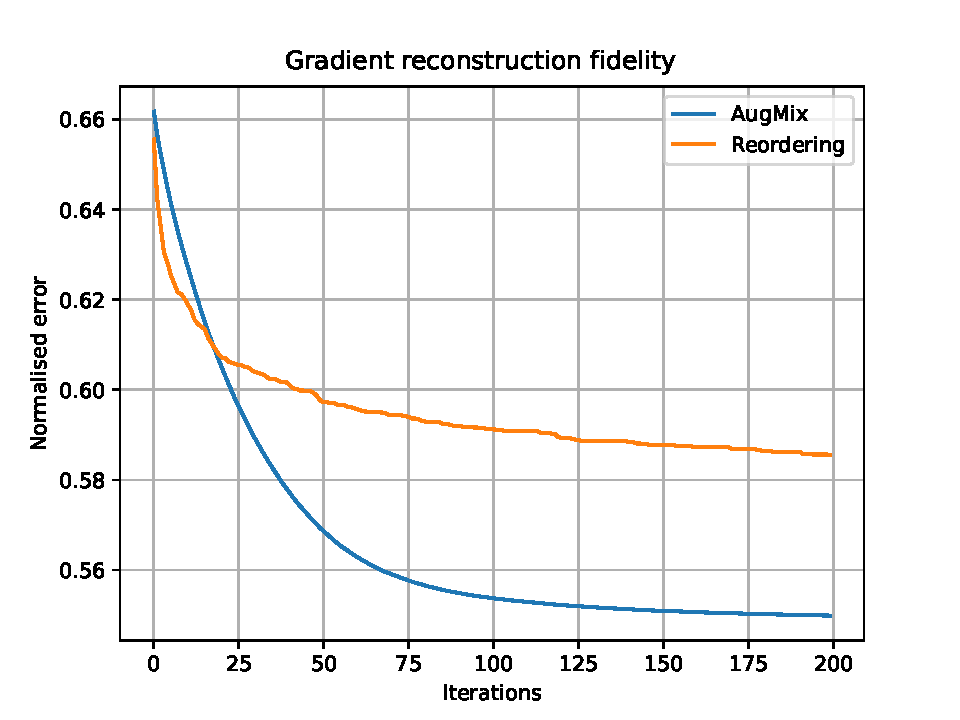
\includegraphics[scale=0.45]{figures/AugMix_error.pdf}
\vspace{-10pt}
\caption{Comparison between our proposed AugMix backdoor and the previous Batch Ordering Backdoor \citep{bob}. The graph shows the averaged reconstruction error over 200 iterations of our AugMix backdoor alongside the error from the Batch Ordering Backdoor. We averaged the errors over 95 sequential batches, trained with the same parameters as for the bottom row of \Cref{tab:augmix}. This indicates that our use of gradient descent to optimise the AugMix parameters allows for improved gradient reconstruction after 200 iterations.}
\label{fig:augmix}
\vspace{-5pt}
\end{figure}

Our AugMix backdoor improves over the previous Batch Order Backdoor in two ways: \textbf{(i)} by providing a mechanism to insert the backdoor into the training pipeline and \textbf{(ii)} by enabling an improved optimisation technique for the gradient shaping process. In this section, we investigate the effect of this second improvement, along with the overall performance of the attack. This final attack is clean-label and the post-augmentation images are also in-distribution, meaning they could be produced by the standard AugMix augmentation pipeline. 

\Cref{fig:augmix} shows the error between our target gradients from an overtly backdoored dataset and our maliciously AugMixed batch. It is clear that our proposed technique allows for improved gradient reconstruction fidelity. We were unable to achieve significant error improvement when using random sampling with our AugMix backdoor, which may be due to the sampling's inability to effectively explore the larger parameter space. The AugMix function's larger parameter space may also correspond to a wider set of possible gradient updates. This improved error is therefore likely due to a combination of the AugMix function's improved lower bound on gradient reconstruction error and our use of gradient descent to more efficiently approach this lower bound.

\begin{table}[!t]
\centering
\caption{Percentage accuracies of classifiers trained on CIFAR10 using our backdoored AugMix function. The trigger we inserted was the flag-like trigger described by \cite{bob}. We performed 200 iterations with Adam optimiser using $\beta=(0.99, 0.999)$ and $1\times10^{-3}$ learning rate to find the AugMix parameters. Following the setup described by \cite{bob}, we initially trained each classifier for 10 clean epochs, followed by 10 adversarially AugMixed batches. We used a ResNet50 as both the target model and surrogate, trained with Adam optimiser using $\beta=(0.99, 0.999)$ and $1\times10^{-3}$ learning rate.}
\label{tab:augmix}
\adjustbox{scale=0.95}{\begin{tabular}{lc||lr|ll}
\toprule

& & \multicolumn{4}{c}{\textbf{CIFAR10}} \\

Attack
& Batch size
& Clean acc. (\%)
& $\Delta$
& Trigger acc. (\%)
& Error w. trigger \\
\midrule
\multirow{3}{*}{None}
& 32 & 84.07 & 0.00 & 13.61 & 27.90 \\
& 64 & 83.96 & 0.00 & 12.94 & 31.16 \\
& 128 & 83.83 & 0.00 & 10.62 & 31.90 \\
\midrule
\multirow{3}{*}{AugMix}
& 32 & 79.73 & -4.34 & 84.73 & 84.19 \\
& 64 & 79.53 & -4.43 & 89.88 & 85.75 \\
& 128 & 79.10 & -4.73 & 95.77 & 88.52 \\ 
\bottomrule
\end{tabular}}
\vspace{-10pt}
\end{table}

\Cref{tab:augmix} presents the results of our AugMix attack. We develop our attack on the codebase from \cite{bob} to make a fair comparison and achieve similar baseline accuracy to them. Our backdoor is able to achieve 95.77\% trigger accuracy. This is a 5.2\% increase in accuracy over the best result achieved by the previous Batch Order Backdoor method. Our results indicate that the attack is most effective on larger batch sizes, which differs from the ordering method, because our attack is able to take advantage of the larger number of parameters more effectively. We performed all of our tests with an AugMix width of 20 as we found that widening past this made the search much less efficient.

Unlike our GAN-based backdoor, our AugMix backdoor produces clean images and labels to insert a backdoor with similar properties to a BadNet. 
Our attack is therefore difficult to directly detect. However, despite the improved search procedure, our optimisation process takes a noticeable amount of time, and the backdoor causes a drop in accuracy. Unlike the GAN-based backdoor, it would be possible to detect this backdoor by careful inspection of the source code. It may be possible to reduce these limitations by using an augmentation that genuinely performs some optimisation as part of the augmentation process, such as AutoAugment \citep{autoaug}.
Overall, we find that:

\begin{itemize}
  \item An attacker can introduce a backdoor into a model using only clean data that has been passed through the AugMix augmentation function.
  \item We can improve the reconstruction fidelity of gradient shaping techniques by using a more efficient optimisation process such as gradient descent.
\end{itemize}